\subsection{Оценки для $\ze(s)$, $\ze'(s)$ и $-\ze'(s)/\ze(s)$ на $\{1\le\si\le2,\,|t|\ge3\}$}

Выполнено
$$
  \hm{\sum_{n=1}^{N}\frac1{n^s}}\leqslant\sum_{n=1}^N\frac1{n^\si}\leqslant
	1+\intlim_1^N\frac{dx}{x^\si}=1+\frac{N^{1-\si}-1}{1-\si}.
$$

\pt{1} При $\si>1$ имеем
\begin{equation}
  \label{zeta <= sigma/(sigma-1)}
  \bm{\ze(s)} \le \lim_{N\to\infty}\left(1+\frac{1-N^{1-\si}}{\si-1}\right) \le 
	1+\frac1{\si-1} = \frac{\si}{\si-1},
\end{equation}
оценка плоха при $\si\to1$.

\pt{2} При $1-\ep\le\si,\,\ep\in(0;1)$ имеем
$$
  \hm{\sum_{n=1}^{N}\frac1{n^s}}\le1+\intlim_1^N\frac{dx}{x^\si}\le
	1+\intlim_1^N\frac{dx}{x^{1-\ep}}=1+\frac{N^\ep-1}{\ep}\le
	1+\frac{N^\ep}{\ep}=C(\ep)\cdot N^\ep=O(N^\ep).
$$

\subsubsection{Оценки для $\ze(s)$ и $\ze'(s)$}

\begin{theorem}
  В области $D:=\{1\le\si\le2,\,|t|\ge3\}$ функции $\ze(s),\,\ze'(s)$ есть $O(|t|^\ep)$.
\end{theorem}
\begin{proof}
  Начнем с $\ze(s)$. При $\si>0$ имеем (\ref{zeta_abel_transform}).

  В области $\{1-\ep\le\si\le3,\,|t|\ge2\}$, содержащей нашу, оценки легко получаются. Выберем $N:=\bs{\bm{t}}$.

  \begin{wrapfigure}{r}{90pt}
    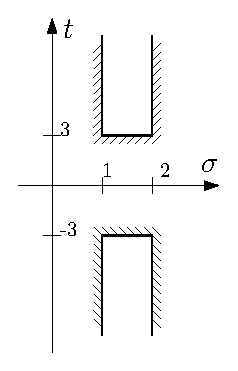
\includegraphics[scale=1.0]{pics/0401}
  \end{wrapfigure}

  \pt{1}
  $$
    \hm{\sum_{n=1}^N\frac1{n^s}}=O(N^\ep)=C_1N^\ep\le C_1|t|^\ep.
  $$

  \pt{2} Имеем $|1-s|=|(1-\si)-it|=\sqrt{(1-\si)^2+t^2}\ge\sqrt{0+4}=2,$ и тогда
  $$
    \hm{\frac{N^{1-s}}{1-s}}\le\frac{N^{1-\si}}{|1-s|}\le\frac{|t|^\ep}2.
  $$

  \pt{3} Используя $|t|-1<N\le|t|$, получаем
  \begin{mlc*}
    \hm{s\intlim_N^\infty\frac{\bc{x}}{x^{s+1}}\,dx} \le
    \sqrt{t^2+9}\intlim_N^\infty\frac{dx}{x^{2-\ep}} \le
    (|t|+3)\left.\frac{x^{\ep-1}}{\ep-1}\right|_N^\infty = \\
    = (|t|+3)\frac{N^\ep N^{-1}}{1-\ep}\le\frac1{1-\ep}\frac{|t|+3}{|t|-1}|t|^\ep \le
    C_2|t|^\ep.
  \end{mlc*}

  Из \pt{1}--\pt{3} следует требуемое.

  Для $\ze'(s)$ воспользуемся формулой Коши:
  $$
    \ze'(s)=\frac1{2\pi i}\intlim_{|z-s|=\ep}\frac{\ze(z)}{(z-s)^2}\,dz,
  $$
  откуда получаем оценку
  %\footnotemark\footnotetext{Почему?}
  $$
    |\ze'(s)|\le\frac1{2\pi}\frac{C_1(|t|+\ep)^\ep}{\ep^2}\le C_2|t|^\ep.
  $$
\end{proof}

Займемся получением такой же оценки для $\frac{\ze'(s)}{\ze(s)}$.

\subsubsection{Лемма о том, что некоторое выражение по модулю не больше $1$}

\begin{lemma}
  При $0<r<1,\,\ph\in\R$
  $$
    M:=\bm{(1-r)^3(1-re^{i\ph})^4(1-re^{2i\ph})}\leqslant1.
  $$
\end{lemma}
\begin{proof}
  \begin{mlc*}
    \ln{M}=3\ln{(1-r)}+4\ln{\bm{1-re^{i\ph}}}+\ln{\bm{1-re^{2i\ph}}}=\\
    =\Re\left(3\ln{(1-r)}+4\ln{(1-re^{i\ph})}+\ln{(1-re^{2i\ph})}\right)=
    -\Re\left(\sum_{n=1}^\infty\frac{r^n}n\left(3+4e^{in\ph}+e^{2in\ph}\right)\right)=\\
    =-\sum_{n=1}^\infty\frac{r^n}n\left(3+4\cos{n\ph}+\cos{2n\ph}\right)=
    -\sum_{n=1}^\infty\frac{r^n}n\cdot2(1+\cos{n\ph})^2\leqslant0.
  \end{mlc*}
  Потенцируя, получаем требуемое.
\end{proof}

\begin{lemma}
  При $\si>1,\,t\in\R$ $$A:=\hm{\ze^3(\si)\ze^4(\si+it)\ze(\si+2it)}\ge1.$$
\end{lemma}
\begin{proof}
  Воспользуемся формулой Эйлера для $\ze(s)$. Тогда получим
  $$
    A=\prod_p\bbbm{\left(1-\frac1{p^\si}\right)^3\left(1-\frac1{p^{\si+it}}\right)^4\left(1-\frac1{p^{\si+2it}}\right)}^{-1}.
  $$

  Выбирая $r:=\frac1{p^\si},\,e^{i\ph}:=p^{-it}$, т.е. $\ph:=-t\ln{p}$, получаем по предыдущей лемме требуемое.
\end{proof}

\subsubsection{Отсутствие нулей $\ze(s)$ в области $\{\si\ge1\}$}

\begin{theorem}
  При $\si\ge1$ $\ze(s)\neq0$.
\end{theorem}
\begin{proof}
  Наше утверждение при $\si>1$ вытекает из последней леммы: если $\ze(s)=0$, то $A=0\ge1$~— противоречие.

  Случай $\si=1$ несколько сложнее.

  Допустим, $\ze(1+it)=0$. Будем считать, что $1<\si<2$.

  \pt{1} Из оценки~(\ref{zeta <= sigma/(sigma-1)})~имеем $0<\ze(\si)\leqslant\frac{\si}{\si-1}<\frac2{\si-1}$.

  \pt{2} В силу непрерывности $\ze(s)$ по $\si$ на $[1;2]$ имеем $|\ze(\si+2it)|\leqslant C_1$.

%   \pt{3} $\ze'(s)=\:?$\footnote{И чему же равно $\ze'(s)$?}, значит, $\limlim_{\si\to1+0}\frac{\ze(\si+it)-\ze(1+it)}{\si-1}=\limlim_{\si\to1+0}\frac{\ze(\si+it)}{\si-1}$, откуда
%   следует, что $\left|\frac{\ze(\si+it)}{\si-1}\right|\leqslant C_2$, т.е. $|\ze(\si+it)|\leqslant C_2|\si-1|$.

  \pt{3} 
	%$\ze'(s)=\:?$\footnote{И чему же равно $\ze'(s)$?}, значит
  $$
    \limlim_{\si\to1+0}\frac{\ze(\si+it)-\ze(1+it)}{\si-1} = \limlim_{\si\to1+0}\frac{\ze(\si+it)}{\si-1} \Rightarrow
    \left|\frac{\ze(\si+it)}{\si-1}\right|\leqslant C_2 \Rightarrow
    |\ze(\si+it)|\leqslant C_2|\si-1|.
  $$

  Тогда
%\footnote{Разъяснить пункты 2, 3.}
  $$
  1\le A\le\left|\left(\frac2{\si-1}\right)^3(C_2(\si-1))^4C_1\right|=C_3|\si-1|\xra{\si\to1+0}0
  $$
  Полученное противоречие доказывает теорему.
\end{proof}

\subsubsection{Оценка для $-\ze'(s)/\ze(s)$}

\begin{theorem}
  В области $D:=\{1\leqslant\si\leqslant2,\,|t|\ge3\}$ $\frac{\ze'(s)}{\ze(s)}$ есть $O(|t|^\ep)$.
\end{theorem}

% \begin{wrapfigure}{r}{120pt}
%   \begin{center}
%   \vskip -50pt
%   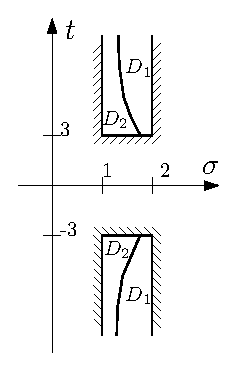
\includegraphics[scale=1.0]{pics/0402}
%   \vskip 10pt
%   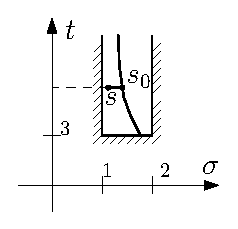
\includegraphics[scale=1.0]{pics/0403}
%   \end{center}
% \end{wrapfigure}

\begin{proof}
  \begin{wrapfigure}{r}{120pt}
    \vskip -40pt
    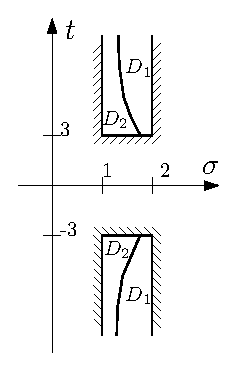
\includegraphics[scale=1.0]{pics/0402}
  \end{wrapfigure}

  Разобьем нашу область на две части $D_1,\,D_2$ по кривой $\si=1+\la|t|^{-\ep}, \la$ определим позднее.

  \pt{1} Пусть $s\in D_1$. По доказанному можем считать, что $|\ze(\si+2it)| \bw\leqslant C_1|t|^{\ep/5}$. Тогда из леммы имеем
  \begin{mlc*}
    |\ze(s)|=|\ze(\si+it)|\ge\ze(\si)^{-3/4}|\ze(\si+2it)|^{-1/4}\ge\\\ge
    \left(\frac2{\la|t|^{-\ep}}\right)^{-3/4}\left(C_1|t|^{\ep/5}\right)^{-1/4}=\widetilde{C_1}\la^{3/4}|t|^{-{4\ep}/5}.
  \end{mlc*}

  \pt{2} Пусть $\si+it=s\in D_2$. Определим $\si_0(t):=1+\la|t|^{-\ep},\,s_0(t):=\si_0(t)+it$.
  Тогда $\intlim_\si^{\si_0}\ze'(x+it)\,dx\bw=\ze(\si_0+it)-\ze(\si+it).$ Заметим, что выполняется оценка
  $\left|\intlim_\si^{\si_0}\ze'(x+it)\,dx\right|\bw\leqslant(\si_0\bw-\si)C_2|t|^{\ep/5}\leqslant\widetilde{C_2}\la|t|^{-\ep}|t|^{\ep/5}=\widetilde{C_2}\la|t|^{-4\ep/5}.$

  \begin{wrapfigure}{r}{120pt}
    \vskip -50pt
    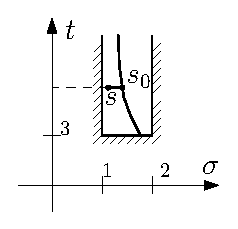
\includegraphics[scale=1.0]{pics/0403}
  \end{wrapfigure}

  Имеем
  \begin{mlc*}
    |\ze(s)|=|\ze(\si+it)|\ge|\ze(\si_0+it)|-\left|\intlim_\si^{\si_0}\ze'(x+it)\,dx\right|\ge \\
    \ge \widetilde{C_1}\la^{3/4}|t|^{-4\ep/5}-\widetilde{C_2}\la|t|^{-4\ep/5}=
    \la^{3/4}\left(\widetilde{C_1}-\widetilde{C_2}\la^{1/4}\right)|t|^{-4\ep/5}.
  \end{mlc*}

  Можем выбрать $\la\colon\widetilde{C_1}-\widetilde{C_2}\la^{1/4}>0.$ Тогда во всей области $D$
  $$
    |\ze(s)|\ge C_3|t|^{-4\ep/5}.
  $$

  Получаем требуемое $$\left|\frac{\ze'(s)}{\ze(s)}\right|\leqslant\frac{C_4|t|^{\ep/5}}{C_3|t|^{-4\ep/5}}=C|t|^\ep.$$
\end{proof} 
